\documentclass[a4paper]{article}


\usepackage[utf8]{inputenc}
\usepackage[T1]{fontenc}
\usepackage{textcomp}
\usepackage{mathtools,amssymb,amsthm}
\usepackage[top=2.5cm,bottom=2.5cm,right=2.5cm,left=2.5cm]{geometry}
\usepackage[francais]{babel}
\usepackage{appendix}

%================image=================
\usepackage{graphicx}
\graphicspath{{figures/}}
\renewcommand{\listfigurename}{Table des figures}

%============header and foot============
\usepackage{fancyhdr}
\pagestyle{fancy}
\renewcommand\headrulewidth{1pt}
\fancyhead[L]{\bfseries Programmation Avancée en C}
\fancyhead[R]{
\includegraphics[scale=0.05]{./img_rapport/prepisima.png}}
\fancyfoot[L]{CLIQUOT Théo et CHASSAGNOL Rémi}
\fancyfoot[R]{2020-2021}

%=================other================
\renewcommand{\contentsname}{Table des matières}

%=================code=================
\usepackage{verbatim}
\usepackage{listings}
\usepackage{color}
\usepackage[table]{xcolor}

%==============code settings==========
\definecolor{darkWhite}{rgb}{1,1,1}
\definecolor{myred}{rgb}{1,0.22,0.22}
\definecolor{mypurple}{rgb}{0.74,0.36,0.97}
\lstset{
  mathescape,
  aboveskip=3mm,
  belowskip=-2mm,
  backgroundcolor=\color{darkWhite},
  basicstyle=\ttfamily\footnotesize,
  breakatwhitespace=false,
  breaklines=true,
  captionpos=b,
  commentstyle=\color{myred},
  deletekeywords={...},
  escapeinside={\%*}{*)},
  extendedchars=true,
  framexleftmargin=16pt,
  framextopmargin=3pt,
  framexbottommargin=6pt,
  frame=tb,
  keepspaces=true,
  keywordstyle=\color{mypurple},
  language=C,
  morekeywords={*,...},
  numbers=left,
  numbersep=10pt,
  numberstyle=\tiny\color{black},
  rulecolor=\color{black},
  showspaces=false,
  showstringspaces=false,
  showtabs=false,
  stepnumber=1,
  stringstyle=\color{gray},
  tabsize=4,
  title=\lstname,
}


\begin{document}

\begin{titlepage}


  \begin{figure}[!htb]
    \begin{minipage}{0.5\textwidth}
      \centering
      
\includegraphics[width=.7\linewidth]{./img_rapport/prepisima.png}
      \caption{ ISIMA }\label{fig-ISIMA}
    \end{minipage}\hfill
    \begin{minipage}{0.5\textwidth}
      \centering
      
\includegraphics[width=.7\linewidth]{./img_rapport/logo.png}
      \caption{Université de Clermont-Ferrand}\label{fig-UCA}
    \end{minipage}
  \end{figure}

  \vspace{2cm}

  \begin{center}


    {\huge \bfseries Projet de Programmation avancée en C\\[0.4cm]}

    \vspace{0.5cm}
    
    {\huge Réalisation d'un jeu de Taquin}

    \vspace{1cm}

    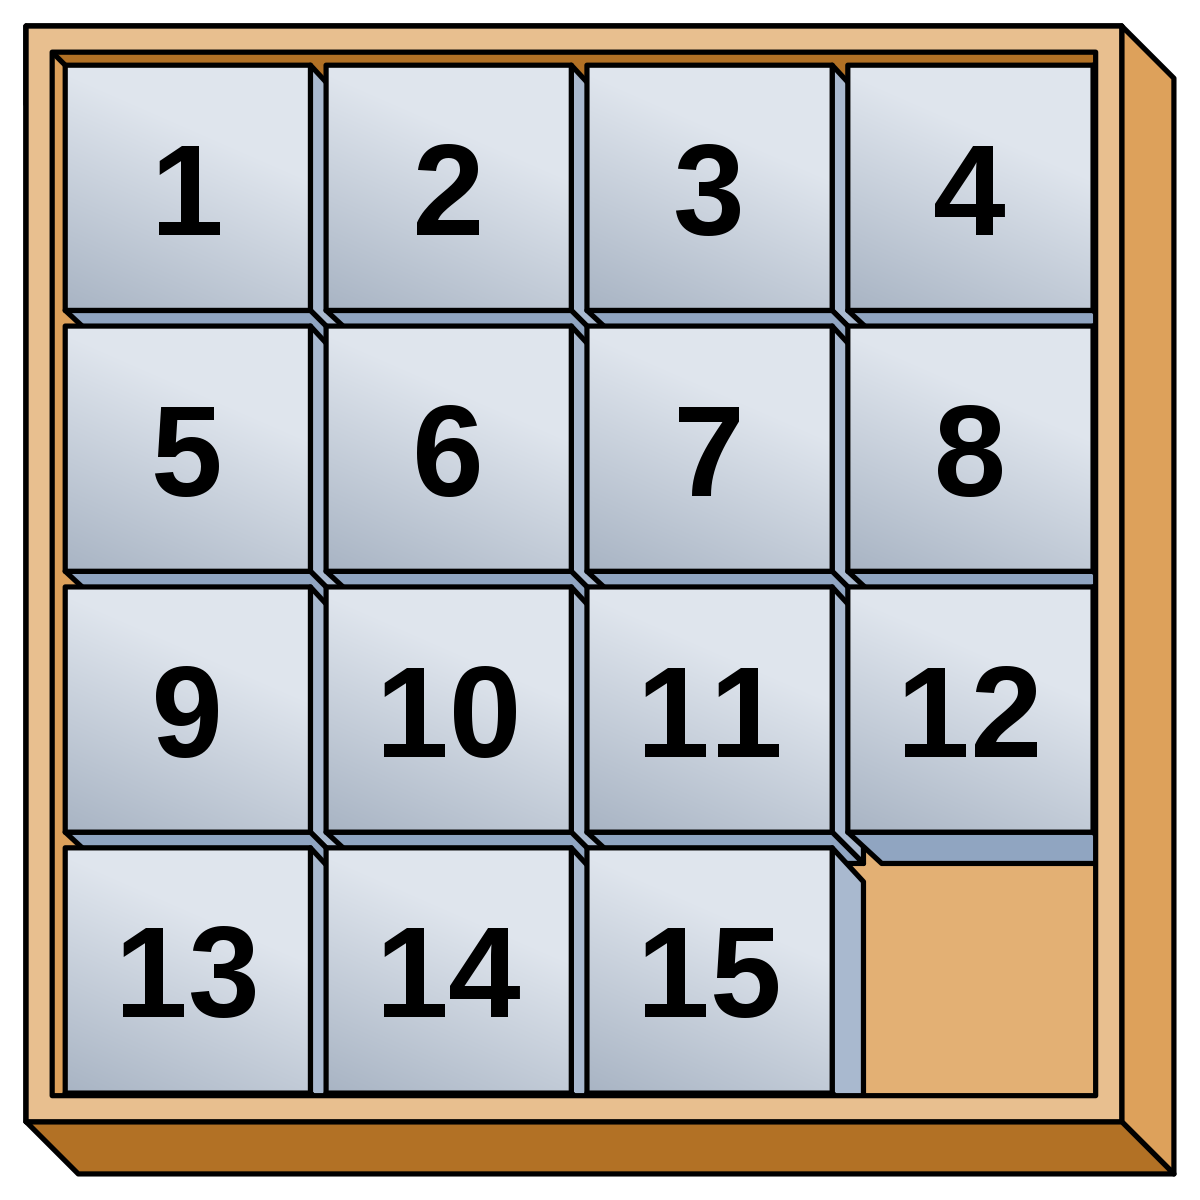
\includegraphics[scale=0.2]{./img_rapport/taquin.png}

    \vspace{1cm}

    \begin{minipage}{0.9\textwidth}
      \begin{flushleft} \large
        CLIQUOT Théo et CHASSAGNOL Rémi\\
        année 2020-2021\\[2cm]
      \end{flushleft}
    \end{minipage}

    \begin{minipage}{0.9\textwidth}
      \begin{flushright} \large
        \emph{Professeurs:} Vincent Limouzy\\
        \emph{Référent TP:} Nicolas Wagner\\
      \end{flushright}
    \end{minipage}

    \vspace{0.5cm}
    
    Travail à rendre pour le : 15/1/2021
    
  \end{titlepage}

  \doublespacing

  \tableofcontents
  \listoffigures

  \doublespacing
  \vspace{2.5cm}

\end{center}

\newpage

\section{Règle du jeux}
\label{sec:regle}


Ce qui va suivre va permettre à n'importe quel personne de jouer au taquin. Cette section contient notamment toutes les touches et toutes les fonctionnalités du jeu. Dès le lancement du jeux on aura d'afficher le taquin, il suffira ensuite d'appuyer sur une touche pour réaliser l'action qu'on veut.


\begin{itemize}
\item Déplacement : Flèches directionnelle.
\item Sauvegarder un taquin : touche \texttt{s}
\item Charger un taquin : Pendant l'appel de l'exécutable donné en argument le nom du fichier.
\item Tarquin aléatoire : Lancé l'exécutable sans autre argument (la taille sera demandé)
\item Tester si le taquin est correcte : touche \texttt{t}
\item ...
\end{itemize}


Les mouvements sont définis par rapport à la case vide , c'est à dire que si on à :
\begin{tabular}{|c|c|c|}
  \hline
  5 &  & 10 \\
  \hline
\end{tabular}
et qu'on appui sur $\triangleright$, on obtiendra :
\begin{tabular}{|c|c|c|}
  \hline
  5 & 10 &   \\
  \hline
\end{tabular}
Et inversement si on appui sur $\triangleleft$, on obtiendra :
\begin{tabular}{|c|c|c|}
  \hline
  & 5 & 10  \\
  \hline
\end{tabular}


\section{Fonctionnement}
\label{sec:fonctionnement}

\subsection{Structure du taquin}
\label{subsec:structTaquin}

On utilise la structure suivante (renommée en texttt{taquin}). textttt{tab} correspond à la postion de nos pièce par rapport à la grille (un tableau 2D),l'entier texttt{posCaseVide} correspond à la position de notre caseVide dans le taquin (par exemple si il est en bas à droite d'un taquin de dimension 5, il sera égale à 24) et enfin l'entier texttt{taille} correspond à la dimension du taquin  :

\begin{lstlisting}
  typedef struct taquin
  {
    int ** tab;
    int posCaseVide;
    int taille;
    
  } taquin;
\end{lstlisting}


\subsection{Sauvegarde du taquin}
\label{subsec:sauv}

Dans cette fonction on sauvegarde dans un fichier de la forme \texttt{sauv txt} notre taquin actuelle. Pour cela on regarde si \texttt{sauv\_0.txt} existe en l'ouvrant . Si il n'existe pas alors on peut créer un fichier représentant le taquin actuelle. Sinon on le ferme et on incrémente notre numéro de sauvegarde (\texttt{sauv\_1.txt}) et ainsi de suite jusqu'à tomber sur un fichier inexistant. Notre taquin est sauvegarder de la façon suivante :
\begin{itemize}
\item Seul le tableau est sauvegarder puisqu'on peut retrouver les autres éléments du taquin à partir de celui-ci.
\item Chaque case du tableau est séparé par un espace.
\item Chaque ligne du tableau est séparé par un saut de ligne.
\end{itemize}

\subsection{Déplacement}
\label{subsec:label}

Pour le déplacement il nous suffit juste d'avoir le taquin est la direction, on regarde si en fonction de la direction que l'on veut notre case vide ne va pas déborder, si ce n'est pas le cas alors on effectue une permutation entre 2 cases (et on oublie pas de mettre à jour la position de la case vide).

\subsection{création du taquin}
\label{subsec:creaTaquin}

\subsubsection{Taquin aléatoire}
\label{subsubsec:creaAlea}
Pour créer un taquin aléatoire selon une taille donnée, il nous suffit de créer un taquin avec un tableau comme on le veut à l'arriver et assigner à \texttt{posCaseVide} et \texttt{taille} la bonne valeur. Puis on applique un certain nombre de fois des déplacementes afin de mélanger le tableau. 

\subsubsection{Taquin charger}
\label{subsubsec:charger}
Il nous suffit de lire un fichier avec la même construction que notre fichier de sauvegarde et récupérer les valeurs de \texttt{tableau}, \texttt{taille} et \texttt{posCaseVide}

\subsection{Taquin Trié}
\label{subsec:taquinTrié}

Il suffit de parcourir le tableau est de regarder si dans la case 0 on à 1, dans la case 1 on à 2 ... et pour la dernière -1.



% Ma Partie

\section{L'affichage SDL}

Il y a en tout cinq fonctions d'affichage pour cinq écran différents. La
première fonction va afficher le message de début de jeu (et le logo), la
seconde va afficher un message qui demande à l’utilisateur si il souhaite
sauvegarder sa progression dans la partie. Les trois autres vont afficher les
écrans de jeu de fin et le menu d'aide.

\subsection{L'affichage Principal}

Cette fonction est la fonction d'affichage principale, elle va afficher les
différentes parties de l'image en fonction de la grille du taquin. Chaque case du
tableau correspond à une certaine partie de l'image en fonction de la valeur
quelle contient. Par exemple, une case qui contient 1 correspond au coin en haut
à gauche de l'image. La taille de la surface de l'image qui correspond à une
case de tableau dépend de la taille de la grille.

Cette fonction utilise une seule surface (sans compter l'écran) qui contient
l'image et deux \textbf{SDL\_Rect}, une  qui sert à découper l'image en plusieurs
partie et l'autre sui sert à coller chacune de ces parties sur l'écran.

\subsection{Les affichages secondaires}
\subsubsection{L'affichage de l'écran de départ}

Cette fonction permet d'afficher le petit texte qui apparaît lorsqu'on lance le
programme. Elle affiche aussi le logo de DOOM en utilisant la fonction
\textbf{SDL\_SerColorKey} et l'option \textbf{SDL\_SRCCOLORKEY} pour ne pas
afficher le fond blanc du logo. Elle fait appel à la fonction attend touche pour
attendre que l'utilisateur appuis sur une touche pour démarrer le jeu et donc
changer l'affichage. Cette fonction retourne un entier pour que l'on puisse
détecter quand l'utilisateur quitte la fenêtre et donc ne pas démarrer le jeu dans
la fonction main.

\subsubsection{Le menu d'aide}

Cette fonction est appelée quand l'utilisateur appuis sur la touche \textbf{escape}
pendant le jeu et affiche un texte qui donne les différents contrôles clavier au
joueur.

\subsubsection{La demande de sauvegarde}

Cette fonction est appelée quand l'utilisateur quitte la fenêtre (en appuyant sur
\textbf{q}) sans avoir fini le jeu. Elle affiche un texte expliquant que
l'utilisateur peut appuyer sur \textbf{y} pour sauvegarder sa partie, toute
autre touche fermera le programme sans sauvegarde. La boucle attendant la
réponse de l'utilisateur se trouve dans la fonction.

\subsubsection{L'affichage de fin}

Cette fonction est appelée quand l'utilisateur a complété le défi et a appuyé
sur \textbf{t} ou \textbf{q}. Elle affiche ``victoire'' et aussi le nombre de
coup que le jour a mis pour terminer le jeu à l'aide \textbf{SDL\_TTF}. Elle fait
appel à la fonction \textbf{attend\_touche} qui permet d'attendre que le joueur
appuis sur une touche pour fermer le programme.

\section{Les contrôles claviers}

Il y a deux fonctions qui permettent de détecter que l'utilisateur appuis sur
des touches du clavier. La fonction attend touche est située dans affichage.h ne
sert que à attendre que l'utilisateur appuis sur une touche et retourne 0 si
l'utilisateur ferme la fenêtre.

L'autre fonction est la fonction de récupération
des touche principal et intervient pendant le jeu. Elle permet à l'utilisateur
de déplacer les pièces en utilisant les flèches (ou les touches de déplacement
de l'éditeur vi), mais aussi de faire apparaître le menu en appuyant sur \textbf{escape},
de quitter le programme en appuyant sur \textbf{q} ou en fermant la fenêtre,
d'activer l'affichage du numéro des pièces ou l'espacement entre les pièces et
enfin de tester si la grille est valide. Cette fonction retourne aussi 0 quand
l'utilisateur quitte la fenêtre.


\end{document}







